\documentclass[letterpaper,11pt]{article}

\usepackage{geometry}
\usepackage{pslatex}
\usepackage{fancyhdr}
\usepackage{graphicx}
\usepackage{color}
\usepackage{tikz}
\usepackage{setspace}
\geometry{ margin = 1.0in }

\pagestyle{fancy}
\lhead{{\bf Lecture 32}}
\chead{{\bf CMPSC 465 Fall 2020}}
\rhead{{\bf Mingfu Shao}}

\setlength\parindent{0em}
\setlength\parskip{8pt}
%\setlength{\fboxsep}{6pt}

\usepackage{amsthm}
\newtheoremstyle{mytheorem}
  {\parskip} % Space above
  {0em} % Space below
  {} % Body font
  {} % Indent amount
  {\bfseries} % Theorem head font
  {.} % Punctuation after theorem head
  {.5em} % Space after theorem head
  {} % Theorem head spec (can be left empty, meaning `normal')

\theoremstyle{mytheorem}
\newtheorem{definition}{Definition}
\newtheorem{property}{Property}
\newtheorem{claim}{Claim}
\newtheorem{fact}{Fact}
\newtheorem{corollary}{Corollary}

% for algorithms
\newcommand{\aaa}[1]{\hspace{0.65cm}\parbox[t]{15.3cm}{#1}}
\newcommand{\aab}[1]{\hspace{1.15cm}\parbox[t]{15.0cm}{#1}}
\newcommand{\aac}[1]{\hspace{1.65cm}\parbox[t]{15.0cm}{#1}}
\newcommand{\aad}[1]{\hspace{2.15cm}\parbox[t]{15.0cm}{#1}}
\newcommand{\aae}[1]{\hspace{2.65cm}\parbox[t]{15.0cm}{#1}}
\newcommand{\aaf}[1]{\hspace{3.15cm}\parbox[t]{15.0cm}{#1}}
\newcommand{\aaA}[2]{\hspace{0.5cm} {\tikz[overlay] \draw (0.1, -0.1) -- (0.1, #1 * -1.5em + 0.6em);} \parbox[t]{15.0cm}{#2}}
\newcommand{\aaB}[2]{\hspace{1.0cm} {\tikz[overlay] \draw (0.1, -0.1) -- (0.1, #1 * -1.5em + 0.6em);} \parbox[t]{15.0cm}{#2}}
\newcommand{\aaC}[2]{\hspace{1.5cm} {\tikz[overlay] \draw (0.1, -0.1) -- (0.1, #1 * -1.5em + 0.6em);} \parbox[t]{15.0cm}{#2}}
\newcommand{\aaD}[2]{\hspace{2.0cm} {\tikz[overlay] \draw (0.1, -0.1) -- (0.1, #1 * -1.5em + 0.6em);} \parbox[t]{15.0cm}{#2}}
\newcommand{\aaE}[2]{\hspace{2.5cm} {\tikz[overlay] \draw (0.1, -0.1) -- (0.1, #1 * -1.5em + 0.6em);} \parbox[t]{15.0cm}{#2}}
\newcommand{\xxx}{\par\vspace{0.1cm}}

\begin{document}

\section*{Disjoint-Set and Its Use in Kruskal's Algorithm}

\subsection*{Disjoint-Set}

A \emph{disjoint-set}, also called \emph{union-find},
is an efficient data structure to store \emph{a collection of disjoint sets}.
In each set, one of the elements is designated as the \emph{representative}
of this set. The representative element serves
as the identity of the set. 
A disjoint-set data structure supports the following operations.
\vspace*{-\topsep}
\begin{enumerate}
\item \emph{make-set~($x$)}, creates a new set with $x$ being the only element.
\item \emph{find~($x$)}, find the set that includes element $x$, by returning the representative of the set.
\item \emph{union~($x$, $y$)}, merge the two sets that include $x$ and $y$.
\end{enumerate}

Note that we can simply decide if two elements $x$ and $y$ are in the same set
by using above \emph{find} function: two elements are in the same set
if and only if they correspond to the same representative, i.e., \emph{find~($x$) $=$ find~($y$)}.

We use a tree to store a set: elements of a set is stored in the nodes of a tree.
The collection of sets is stored with a \emph{forest}~(i.e., a collection of trees).
The reason we use trees to store sets is that, the \emph{union} operation
can be easily implemented by simply merging two trees.
We also store the \emph{height} of each subtree.
(The height of a subtree rooted at node $v$ is defined as the length of the longest path 
from $v$ to a leaf node.) The reason we store heights is to maintain a \emph{balanced} tree
as much as possible---we don't want the tree to be too tall, as the running time
of \emph{find} operation is proportional to the height of the tree~(see below).
An implementation of the \emph{node} class of a tree will look like this~(in C++):

\begin{minipage}{0.8\textwidth}
	\aaa {class node~\{}\xxx
	\aab {void* data; \ // storing the actual data}\xxx
	\aab {int height; \ // storing the height of the subtree rooted at this node}\xxx
	\aab {node* parent; \ // pointer to the parent node of this node}\xxx
	\aaa {\};}\xxx
\end{minipage}

We define the root of each tree always being the representative of the corresponding set.
And we always use a pointer that points to itself, i.e., $x.parent = x$, to label
that a node is a root.
Below we give the pseudo-code for these 3 operations.
We assume that elements~($x$, $y$, etc, used below) are with above \emph{node} type.

\begin{minipage}{0.8\textwidth}
	\aaA {3}{function make-set~($x$)}\xxx
	\aab {$x.height = 1$;}\xxx
	\aab {$x.parent = x$;}\xxx
	\aaa {end;}\xxx
\end{minipage}

The \emph{find} operation traverses the path following the parent pointers 
until reaching the root. Note that the running time of this procedure
is propotional to the height of the tree.

\begin{minipage}{0.8\textwidth}
	\aaA {5}{function find~($x$)}\xxx
	\aaB {2}{while~($x.parent \neq x$)}\xxx
	\aac {$x = x.parent$;}\xxx
	\aab {end;}\xxx
	\aab {return $x$;}\xxx
	\aaa {end;}\xxx
\end{minipage}

The union operation first find the roots of the two trees that contains $x$ and
$y$ respectively, and then merge them by hanging one of the tree under the root
of the other tree. Notice that we want the tree as shorter as possible;
hence we always hang the shorter tree under the taller tree~(break tie arbitrarily when equal).
Note too that if the two trees have different heights,
after merging all heights remain the same;
if the two trees have the same height, then after merging
the height of the new root will be increased by 1.
See Figure~\ref{fig:union}.

\begin{minipage}{0.8\textwidth}
	\aaA {12}{function union~($x,y$)}\xxx
	\aab {$r_x = find(x)$;}\xxx
	\aab {$r_y = find(y)$;}\xxx
	\aab {if~($r_x = r_y$): return; \ // $x$ and $y$ already in the same tree}\xxx
	\aaB {2}{if~($r_x.height < r_y.height$)}\xxx
	\aac {$r_x.parent = r_y$}\xxx
	\aaB {2}{else if~($r_x.height > r_y.height$)}\xxx
	\aac {$r_y.parent = r_x$}\xxx
	\aaB {3}{else}\xxx
	\aac {$r_x.parent = r_y$}\xxx
	\aac {$r_y.height = r_y.height + 1$}\xxx
	\aab {end}\xxx
	\aaa {end;}\xxx
\end{minipage}


\begin{figure}[h]
\centering{

\tikzset{every picture/.style={line width=0.75pt}} %set default line width to 0.75pt        

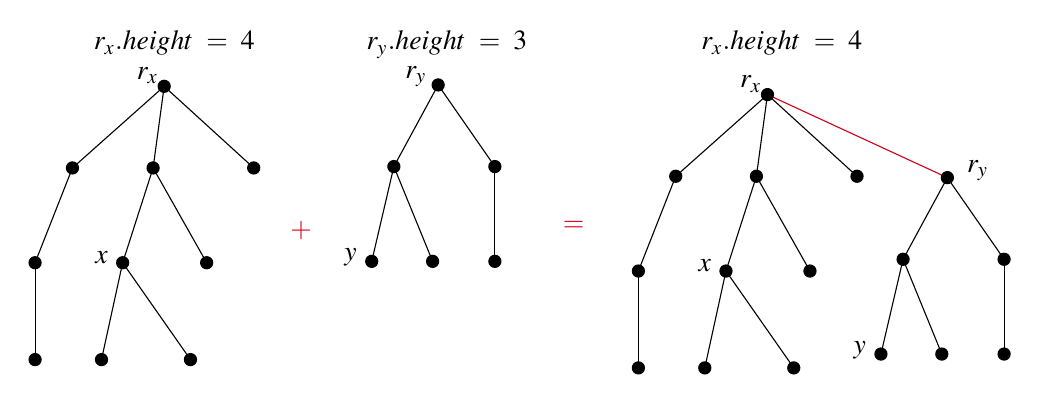
\begin{tikzpicture}[x=0.5pt,y=0.5pt,yscale=-1,xscale=1]
%uncomment if require: \path (0,281); %set diagram left start at 0, and has height of 281

%Flowchart: Connector [id:dp9897896441945839] 
\draw  [fill={rgb, 255:red, 0; green, 0; blue, 0 }  ,fill opacity=1 ] (105.59,53.9) .. controls (106.45,51.65) and (108.99,50.52) .. (111.24,51.39) .. controls (113.5,52.26) and (114.62,54.79) .. (113.75,57.05) .. controls (112.88,59.3) and (110.35,60.43) .. (108.1,59.56) .. controls (105.84,58.69) and (104.72,56.16) .. (105.59,53.9) -- cycle ;
%Flowchart: Connector [id:dp8075110738416615] 
\draw  [fill={rgb, 255:red, 0; green, 0; blue, 0 }  ,fill opacity=1 ] (39.29,112.9) .. controls (40.16,110.65) and (42.69,109.52) .. (44.95,110.39) .. controls (47.2,111.26) and (48.33,113.79) .. (47.46,116.05) .. controls (46.59,118.3) and (44.06,119.43) .. (41.8,118.56) .. controls (39.55,117.69) and (38.42,115.16) .. (39.29,112.9) -- cycle ;
%Straight Lines [id:da9902964456425614] 
\draw [color={rgb, 255:red, 208; green, 2; blue, 27 }  ,draw opacity=1 ]   (545.67,61.48) -- (675.67,121.48) ;
%Straight Lines [id:da5172177882024809] 
\draw    (43.37,114.48) -- (109.67,55.48) ;
%Flowchart: Connector [id:dp11019606064742127] 
\draw  [fill={rgb, 255:red, 0; green, 0; blue, 0 }  ,fill opacity=1 ] (97.59,112.9) .. controls (98.45,110.65) and (100.99,109.52) .. (103.24,110.39) .. controls (105.5,111.26) and (106.62,113.79) .. (105.75,116.05) .. controls (104.88,118.3) and (102.35,119.43) .. (100.1,118.56) .. controls (97.84,117.69) and (96.72,115.16) .. (97.59,112.9) -- cycle ;
%Flowchart: Connector [id:dp28900689737394614] 
\draw  [fill={rgb, 255:red, 0; green, 0; blue, 0 }  ,fill opacity=1 ] (170.29,112.9) .. controls (171.16,110.65) and (173.69,109.52) .. (175.95,110.39) .. controls (178.2,111.26) and (179.33,113.79) .. (178.46,116.05) .. controls (177.59,118.3) and (175.06,119.43) .. (172.8,118.56) .. controls (170.55,117.69) and (169.42,115.16) .. (170.29,112.9) -- cycle ;
%Flowchart: Connector [id:dp8349300680889286] 
\draw  [fill={rgb, 255:red, 0; green, 0; blue, 0 }  ,fill opacity=1 ] (75.59,181.4) .. controls (76.45,179.15) and (78.99,178.02) .. (81.24,178.89) .. controls (83.5,179.76) and (84.62,182.29) .. (83.75,184.55) .. controls (82.88,186.8) and (80.35,187.93) .. (78.1,187.06) .. controls (75.84,186.19) and (74.72,183.66) .. (75.59,181.4) -- cycle ;
%Flowchart: Connector [id:dp5271991889149706] 
\draw  [fill={rgb, 255:red, 0; green, 0; blue, 0 }  ,fill opacity=1 ] (12.29,181.4) .. controls (13.16,179.15) and (15.69,178.02) .. (17.95,178.89) .. controls (20.2,179.76) and (21.33,182.29) .. (20.46,184.55) .. controls (19.59,186.8) and (17.06,187.93) .. (14.8,187.06) .. controls (12.55,186.19) and (11.42,183.66) .. (12.29,181.4) -- cycle ;
%Flowchart: Connector [id:dp4031153203734361] 
\draw  [fill={rgb, 255:red, 0; green, 0; blue, 0 }  ,fill opacity=1 ] (12.29,251.4) .. controls (13.16,249.15) and (15.69,248.02) .. (17.95,248.89) .. controls (20.2,249.76) and (21.33,252.29) .. (20.46,254.55) .. controls (19.59,256.8) and (17.06,257.93) .. (14.8,257.06) .. controls (12.55,256.19) and (11.42,253.66) .. (12.29,251.4) -- cycle ;
%Flowchart: Connector [id:dp0008363872359773428] 
\draw  [fill={rgb, 255:red, 0; green, 0; blue, 0 }  ,fill opacity=1 ] (136.29,181.4) .. controls (137.16,179.15) and (139.69,178.02) .. (141.95,178.89) .. controls (144.2,179.76) and (145.33,182.29) .. (144.46,184.55) .. controls (143.59,186.8) and (141.06,187.93) .. (138.8,187.06) .. controls (136.55,186.19) and (135.42,183.66) .. (136.29,181.4) -- cycle ;
%Flowchart: Connector [id:dp7716868638159723] 
\draw  [fill={rgb, 255:red, 0; green, 0; blue, 0 }  ,fill opacity=1 ] (124.59,251.4) .. controls (125.45,249.15) and (127.99,248.02) .. (130.24,248.89) .. controls (132.5,249.76) and (133.62,252.29) .. (132.75,254.55) .. controls (131.88,256.8) and (129.35,257.93) .. (127.1,257.06) .. controls (124.84,256.19) and (123.72,253.66) .. (124.59,251.4) -- cycle ;
%Flowchart: Connector [id:dp8451689968178246] 
\draw  [fill={rgb, 255:red, 0; green, 0; blue, 0 }  ,fill opacity=1 ] (60.29,251.4) .. controls (61.16,249.15) and (63.69,248.02) .. (65.95,248.89) .. controls (68.2,249.76) and (69.33,252.29) .. (68.46,254.55) .. controls (67.59,256.8) and (65.06,257.93) .. (62.8,257.06) .. controls (60.55,256.19) and (59.42,253.66) .. (60.29,251.4) -- cycle ;
%Flowchart: Connector [id:dp032017927511610256] 
\draw  [fill={rgb, 255:red, 0; green, 0; blue, 0 }  ,fill opacity=1 ] (303.59,52.9) .. controls (304.45,50.65) and (306.99,49.52) .. (309.24,50.39) .. controls (311.5,51.26) and (312.62,53.79) .. (311.75,56.05) .. controls (310.88,58.3) and (308.35,59.43) .. (306.1,58.56) .. controls (303.84,57.69) and (302.72,55.16) .. (303.59,52.9) -- cycle ;
%Flowchart: Connector [id:dp7753230180353938] 
\draw  [fill={rgb, 255:red, 0; green, 0; blue, 0 }  ,fill opacity=1 ] (271.59,111.9) .. controls (272.45,109.65) and (274.99,108.52) .. (277.24,109.39) .. controls (279.5,110.26) and (280.62,112.79) .. (279.75,115.05) .. controls (278.88,117.3) and (276.35,118.43) .. (274.1,117.56) .. controls (271.84,116.69) and (270.72,114.16) .. (271.59,111.9) -- cycle ;
%Flowchart: Connector [id:dp7480294214835582] 
\draw  [fill={rgb, 255:red, 0; green, 0; blue, 0 }  ,fill opacity=1 ] (255.59,180.4) .. controls (256.45,178.15) and (258.99,177.02) .. (261.24,177.89) .. controls (263.5,178.76) and (264.62,181.29) .. (263.75,183.55) .. controls (262.88,185.8) and (260.35,186.93) .. (258.1,186.06) .. controls (255.84,185.19) and (254.72,182.66) .. (255.59,180.4) -- cycle ;
%Flowchart: Connector [id:dp4873571062167924] 
\draw  [fill={rgb, 255:red, 0; green, 0; blue, 0 }  ,fill opacity=1 ] (344.59,111.9) .. controls (345.45,109.65) and (347.99,108.52) .. (350.24,109.39) .. controls (352.5,110.26) and (353.62,112.79) .. (352.75,115.05) .. controls (351.88,117.3) and (349.35,118.43) .. (347.1,117.56) .. controls (344.84,116.69) and (343.72,114.16) .. (344.59,111.9) -- cycle ;
%Flowchart: Connector [id:dp4230951468351575] 
\draw  [fill={rgb, 255:red, 0; green, 0; blue, 0 }  ,fill opacity=1 ] (344.59,180.4) .. controls (345.45,178.15) and (347.99,177.02) .. (350.24,177.89) .. controls (352.5,178.76) and (353.62,181.29) .. (352.75,183.55) .. controls (351.88,185.8) and (349.35,186.93) .. (347.1,186.06) .. controls (344.84,185.19) and (343.72,182.66) .. (344.59,180.4) -- cycle ;
%Flowchart: Connector [id:dp02723705167497803] 
\draw  [fill={rgb, 255:red, 0; green, 0; blue, 0 }  ,fill opacity=1 ] (299.59,180.4) .. controls (300.45,178.15) and (302.99,177.02) .. (305.24,177.89) .. controls (307.5,178.76) and (308.62,181.29) .. (307.75,183.55) .. controls (306.88,185.8) and (304.35,186.93) .. (302.1,186.06) .. controls (299.84,185.19) and (298.72,182.66) .. (299.59,180.4) -- cycle ;
%Straight Lines [id:da8485530944868279] 
\draw    (16.37,182.98) -- (43.37,114.48) ;
%Straight Lines [id:da936425631795308] 
\draw    (79.67,182.98) -- (101.67,114.48) ;
%Straight Lines [id:da3467674009082027] 
\draw    (101.67,114.48) -- (109.67,55.48) ;
%Straight Lines [id:da2710068544626746] 
\draw    (174.37,114.48) -- (109.67,55.48) ;
%Straight Lines [id:da18129286507358067] 
\draw    (140.37,182.98) -- (101.67,114.48) ;
%Straight Lines [id:da44262512432909795] 
\draw    (16.37,252.98) -- (16.37,182.98) ;
%Straight Lines [id:da31047061197895953] 
\draw    (64.37,252.98) -- (79.67,182.98) ;
%Straight Lines [id:da7822071001867994] 
\draw    (128.67,252.98) -- (79.67,182.98) ;
%Straight Lines [id:da8032171189474756] 
\draw    (275.67,113.48) -- (307.67,54.48) ;
%Straight Lines [id:da8169278171705383] 
\draw    (259.67,181.98) -- (275.67,113.48) ;
%Straight Lines [id:da4835943452382059] 
\draw    (303.67,181.98) -- (275.67,113.48) ;
%Straight Lines [id:da6486207879374191] 
\draw    (348.67,113.48) -- (307.67,54.48) ;
%Straight Lines [id:da5877844887696961] 
\draw    (348.67,181.98) -- (348.67,113.48) ;
%Flowchart: Connector [id:dp20762635887871939] 
\draw  [fill={rgb, 255:red, 0; green, 0; blue, 0 }  ,fill opacity=1 ] (541.59,59.9) .. controls (542.45,57.65) and (544.99,56.52) .. (547.24,57.39) .. controls (549.5,58.26) and (550.62,60.79) .. (549.75,63.05) .. controls (548.88,65.3) and (546.35,66.43) .. (544.1,65.56) .. controls (541.84,64.69) and (540.72,62.16) .. (541.59,59.9) -- cycle ;
%Flowchart: Connector [id:dp5761285936520872] 
\draw  [fill={rgb, 255:red, 0; green, 0; blue, 0 }  ,fill opacity=1 ] (475.29,118.9) .. controls (476.16,116.65) and (478.69,115.52) .. (480.95,116.39) .. controls (483.2,117.26) and (484.33,119.79) .. (483.46,122.05) .. controls (482.59,124.3) and (480.06,125.43) .. (477.8,124.56) .. controls (475.55,123.69) and (474.42,121.16) .. (475.29,118.9) -- cycle ;
%Straight Lines [id:da47437536489118703] 
\draw    (479.37,120.48) -- (545.67,61.48) ;
%Flowchart: Connector [id:dp9973180956089771] 
\draw  [fill={rgb, 255:red, 0; green, 0; blue, 0 }  ,fill opacity=1 ] (533.59,118.9) .. controls (534.45,116.65) and (536.99,115.52) .. (539.24,116.39) .. controls (541.5,117.26) and (542.62,119.79) .. (541.75,122.05) .. controls (540.88,124.3) and (538.35,125.43) .. (536.1,124.56) .. controls (533.84,123.69) and (532.72,121.16) .. (533.59,118.9) -- cycle ;
%Flowchart: Connector [id:dp7887397130476378] 
\draw  [fill={rgb, 255:red, 0; green, 0; blue, 0 }  ,fill opacity=1 ] (606.29,118.9) .. controls (607.16,116.65) and (609.69,115.52) .. (611.95,116.39) .. controls (614.2,117.26) and (615.33,119.79) .. (614.46,122.05) .. controls (613.59,124.3) and (611.06,125.43) .. (608.8,124.56) .. controls (606.55,123.69) and (605.42,121.16) .. (606.29,118.9) -- cycle ;
%Flowchart: Connector [id:dp9416096601548867] 
\draw  [fill={rgb, 255:red, 0; green, 0; blue, 0 }  ,fill opacity=1 ] (511.59,187.4) .. controls (512.45,185.15) and (514.99,184.02) .. (517.24,184.89) .. controls (519.5,185.76) and (520.62,188.29) .. (519.75,190.55) .. controls (518.88,192.8) and (516.35,193.93) .. (514.1,193.06) .. controls (511.84,192.19) and (510.72,189.66) .. (511.59,187.4) -- cycle ;
%Flowchart: Connector [id:dp3290524933044451] 
\draw  [fill={rgb, 255:red, 0; green, 0; blue, 0 }  ,fill opacity=1 ] (448.29,187.4) .. controls (449.16,185.15) and (451.69,184.02) .. (453.95,184.89) .. controls (456.2,185.76) and (457.33,188.29) .. (456.46,190.55) .. controls (455.59,192.8) and (453.06,193.93) .. (450.8,193.06) .. controls (448.55,192.19) and (447.42,189.66) .. (448.29,187.4) -- cycle ;
%Flowchart: Connector [id:dp0667118668486314] 
\draw  [fill={rgb, 255:red, 0; green, 0; blue, 0 }  ,fill opacity=1 ] (448.29,257.4) .. controls (449.16,255.15) and (451.69,254.02) .. (453.95,254.89) .. controls (456.2,255.76) and (457.33,258.29) .. (456.46,260.55) .. controls (455.59,262.8) and (453.06,263.93) .. (450.8,263.06) .. controls (448.55,262.19) and (447.42,259.66) .. (448.29,257.4) -- cycle ;
%Flowchart: Connector [id:dp9716822322363012] 
\draw  [fill={rgb, 255:red, 0; green, 0; blue, 0 }  ,fill opacity=1 ] (572.29,187.4) .. controls (573.16,185.15) and (575.69,184.02) .. (577.95,184.89) .. controls (580.2,185.76) and (581.33,188.29) .. (580.46,190.55) .. controls (579.59,192.8) and (577.06,193.93) .. (574.8,193.06) .. controls (572.55,192.19) and (571.42,189.66) .. (572.29,187.4) -- cycle ;
%Flowchart: Connector [id:dp48717164529435164] 
\draw  [fill={rgb, 255:red, 0; green, 0; blue, 0 }  ,fill opacity=1 ] (560.59,257.4) .. controls (561.45,255.15) and (563.99,254.02) .. (566.24,254.89) .. controls (568.5,255.76) and (569.62,258.29) .. (568.75,260.55) .. controls (567.88,262.8) and (565.35,263.93) .. (563.1,263.06) .. controls (560.84,262.19) and (559.72,259.66) .. (560.59,257.4) -- cycle ;
%Flowchart: Connector [id:dp18114130792127026] 
\draw  [fill={rgb, 255:red, 0; green, 0; blue, 0 }  ,fill opacity=1 ] (496.29,257.4) .. controls (497.16,255.15) and (499.69,254.02) .. (501.95,254.89) .. controls (504.2,255.76) and (505.33,258.29) .. (504.46,260.55) .. controls (503.59,262.8) and (501.06,263.93) .. (498.8,263.06) .. controls (496.55,262.19) and (495.42,259.66) .. (496.29,257.4) -- cycle ;
%Flowchart: Connector [id:dp7518877314640476] 
\draw  [fill={rgb, 255:red, 0; green, 0; blue, 0 }  ,fill opacity=1 ] (671.59,119.9) .. controls (672.45,117.65) and (674.99,116.52) .. (677.24,117.39) .. controls (679.5,118.26) and (680.62,120.79) .. (679.75,123.05) .. controls (678.88,125.3) and (676.35,126.43) .. (674.1,125.56) .. controls (671.84,124.69) and (670.72,122.16) .. (671.59,119.9) -- cycle ;
%Flowchart: Connector [id:dp599431917297237] 
\draw  [fill={rgb, 255:red, 0; green, 0; blue, 0 }  ,fill opacity=1 ] (639.59,178.9) .. controls (640.45,176.65) and (642.99,175.52) .. (645.24,176.39) .. controls (647.5,177.26) and (648.62,179.79) .. (647.75,182.05) .. controls (646.88,184.3) and (644.35,185.43) .. (642.1,184.56) .. controls (639.84,183.69) and (638.72,181.16) .. (639.59,178.9) -- cycle ;
%Flowchart: Connector [id:dp16343923312842312] 
\draw  [fill={rgb, 255:red, 0; green, 0; blue, 0 }  ,fill opacity=1 ] (623.59,247.4) .. controls (624.45,245.15) and (626.99,244.02) .. (629.24,244.89) .. controls (631.5,245.76) and (632.62,248.29) .. (631.75,250.55) .. controls (630.88,252.8) and (628.35,253.93) .. (626.1,253.06) .. controls (623.84,252.19) and (622.72,249.66) .. (623.59,247.4) -- cycle ;
%Flowchart: Connector [id:dp6848727750904735] 
\draw  [fill={rgb, 255:red, 0; green, 0; blue, 0 }  ,fill opacity=1 ] (712.59,178.9) .. controls (713.45,176.65) and (715.99,175.52) .. (718.24,176.39) .. controls (720.5,177.26) and (721.62,179.79) .. (720.75,182.05) .. controls (719.88,184.3) and (717.35,185.43) .. (715.1,184.56) .. controls (712.84,183.69) and (711.72,181.16) .. (712.59,178.9) -- cycle ;
%Flowchart: Connector [id:dp8120790196669959] 
\draw  [fill={rgb, 255:red, 0; green, 0; blue, 0 }  ,fill opacity=1 ] (712.59,247.4) .. controls (713.45,245.15) and (715.99,244.02) .. (718.24,244.89) .. controls (720.5,245.76) and (721.62,248.29) .. (720.75,250.55) .. controls (719.88,252.8) and (717.35,253.93) .. (715.1,253.06) .. controls (712.84,252.19) and (711.72,249.66) .. (712.59,247.4) -- cycle ;
%Flowchart: Connector [id:dp3775740881604551] 
\draw  [fill={rgb, 255:red, 0; green, 0; blue, 0 }  ,fill opacity=1 ] (667.59,247.4) .. controls (668.45,245.15) and (670.99,244.02) .. (673.24,244.89) .. controls (675.5,245.76) and (676.62,248.29) .. (675.75,250.55) .. controls (674.88,252.8) and (672.35,253.93) .. (670.1,253.06) .. controls (667.84,252.19) and (666.72,249.66) .. (667.59,247.4) -- cycle ;
%Straight Lines [id:da001803532705640376] 
\draw    (452.37,188.98) -- (479.37,120.48) ;
%Straight Lines [id:da647457490609615] 
\draw    (515.67,188.98) -- (537.67,120.48) ;
%Straight Lines [id:da4980390431112198] 
\draw    (537.67,120.48) -- (545.67,61.48) ;
%Straight Lines [id:da6214247879507085] 
\draw    (610.37,120.48) -- (545.67,61.48) ;
%Straight Lines [id:da10843359313978695] 
\draw    (576.37,188.98) -- (537.67,120.48) ;
%Straight Lines [id:da41275684445149585] 
\draw    (452.37,258.98) -- (452.37,188.98) ;
%Straight Lines [id:da1532167517032782] 
\draw    (500.37,258.98) -- (515.67,188.98) ;
%Straight Lines [id:da9072254965197083] 
\draw    (564.67,258.98) -- (515.67,188.98) ;
%Straight Lines [id:da49132027020689406] 
\draw    (643.67,180.48) -- (675.67,121.48) ;
%Straight Lines [id:da5453594011228895] 
\draw    (627.67,248.98) -- (643.67,180.48) ;
%Straight Lines [id:da9542661262103859] 
\draw    (671.67,248.98) -- (643.67,180.48) ;
%Straight Lines [id:da6774988416466069] 
\draw    (716.67,180.48) -- (675.67,121.48) ;
%Straight Lines [id:da1951736113047675] 
\draw    (716.67,248.98) -- (716.67,180.48) ;

% Text Node
\draw (58,173) node [anchor=north west][inner sep=0.75pt]   [align=left] {$\displaystyle x$};
% Text Node
\draw (88,40) node [anchor=north west][inner sep=0.75pt]   [align=left] {$\displaystyle r_{x}$};
% Text Node
\draw (238,171) node [anchor=north west][inner sep=0.75pt]   [align=left] {$\displaystyle y$};
% Text Node
\draw (282,39) node [anchor=north west][inner sep=0.75pt]   [align=left] {$\displaystyle r_{y}$};
% Text Node
\draw (494,179) node [anchor=north west][inner sep=0.75pt]   [align=left] {$\displaystyle x$};
% Text Node
\draw (524,46) node [anchor=north west][inner sep=0.75pt]   [align=left] {$\displaystyle r_{x}$};
% Text Node
\draw (606,238) node [anchor=north west][inner sep=0.75pt]   [align=left] {$\displaystyle y$};
% Text Node
\draw (688,107) node [anchor=north west][inner sep=0.75pt]   [align=left] {$\displaystyle r_{y}$};
% Text Node
\draw (199,151) node [anchor=north west][inner sep=0.75pt]   [align=left] {$\displaystyle \textcolor[rgb]{0.82,0.01,0.11}{+}$};
% Text Node
\draw (396,151) node [anchor=north west][inner sep=0.75pt]   [align=left] {$\displaystyle \textcolor[rgb]{0.82,0.01,0.11}{=}$};
% Text Node
\draw (57,13.5) node [anchor=north west][inner sep=0.75pt]   [align=left] {$\displaystyle r_{x} .height\ =\ 4$};
% Text Node
\draw (254,13.5) node [anchor=north west][inner sep=0.75pt]   [align=left] {$\displaystyle r_{y} .height\ =\ 3$};
% Text Node
\draw (496,13.5) node [anchor=north west][inner sep=0.75pt]   [align=left] {$\displaystyle r_{x} .height\ =\ 4$};


\end{tikzpicture}

}
\vspace*{0.4cm}
\centering{

\tikzset{every picture/.style={line width=0.75pt}} %set default line width to 0.75pt        

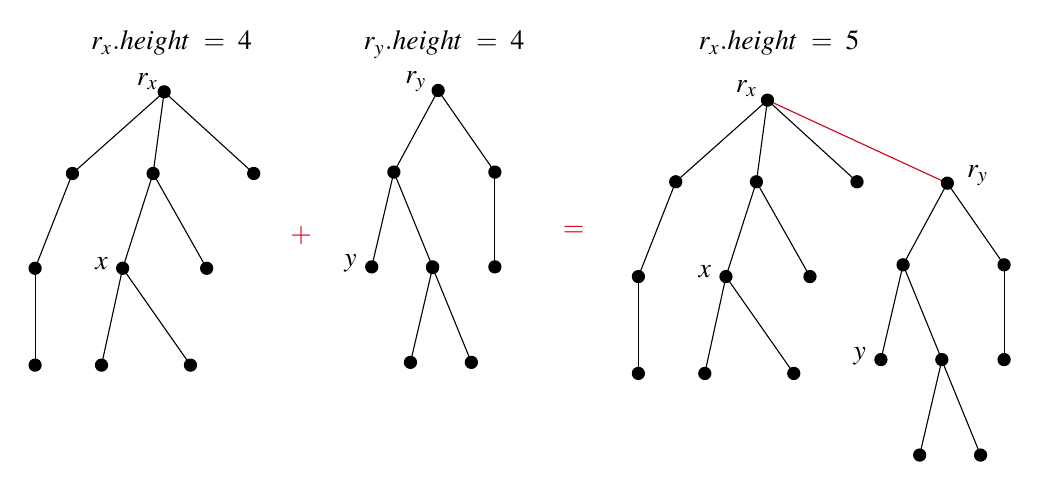
\begin{tikzpicture}[x=0.5pt,y=0.5pt,yscale=-1,xscale=1]
%uncomment if require: \path (0,327); %set diagram left start at 0, and has height of 327

%Flowchart: Connector [id:dp8194762305551321] 
\draw  [fill={rgb, 255:red, 0; green, 0; blue, 0 }  ,fill opacity=1 ] (101.59,50.9) .. controls (102.45,48.65) and (104.99,47.52) .. (107.24,48.39) .. controls (109.5,49.26) and (110.62,51.79) .. (109.75,54.05) .. controls (108.88,56.3) and (106.35,57.43) .. (104.1,56.56) .. controls (101.84,55.69) and (100.72,53.16) .. (101.59,50.9) -- cycle ;
%Flowchart: Connector [id:dp36013323711070966] 
\draw  [fill={rgb, 255:red, 0; green, 0; blue, 0 }  ,fill opacity=1 ] (35.29,109.9) .. controls (36.16,107.65) and (38.69,106.52) .. (40.95,107.39) .. controls (43.2,108.26) and (44.33,110.79) .. (43.46,113.05) .. controls (42.59,115.3) and (40.06,116.43) .. (37.8,115.56) .. controls (35.55,114.69) and (34.42,112.16) .. (35.29,109.9) -- cycle ;
%Straight Lines [id:da7255221211203402] 
\draw [color={rgb, 255:red, 208; green, 2; blue, 27 }  ,draw opacity=1 ]   (541.67,58.48) -- (671.67,118.48) ;
%Straight Lines [id:da7953688832192422] 
\draw    (39.37,111.48) -- (105.67,52.48) ;
%Flowchart: Connector [id:dp8112463194308399] 
\draw  [fill={rgb, 255:red, 0; green, 0; blue, 0 }  ,fill opacity=1 ] (93.59,109.9) .. controls (94.45,107.65) and (96.99,106.52) .. (99.24,107.39) .. controls (101.5,108.26) and (102.62,110.79) .. (101.75,113.05) .. controls (100.88,115.3) and (98.35,116.43) .. (96.1,115.56) .. controls (93.84,114.69) and (92.72,112.16) .. (93.59,109.9) -- cycle ;
%Flowchart: Connector [id:dp4034124904883707] 
\draw  [fill={rgb, 255:red, 0; green, 0; blue, 0 }  ,fill opacity=1 ] (166.29,109.9) .. controls (167.16,107.65) and (169.69,106.52) .. (171.95,107.39) .. controls (174.2,108.26) and (175.33,110.79) .. (174.46,113.05) .. controls (173.59,115.3) and (171.06,116.43) .. (168.8,115.56) .. controls (166.55,114.69) and (165.42,112.16) .. (166.29,109.9) -- cycle ;
%Flowchart: Connector [id:dp7496807460147518] 
\draw  [fill={rgb, 255:red, 0; green, 0; blue, 0 }  ,fill opacity=1 ] (71.59,178.4) .. controls (72.45,176.15) and (74.99,175.02) .. (77.24,175.89) .. controls (79.5,176.76) and (80.62,179.29) .. (79.75,181.55) .. controls (78.88,183.8) and (76.35,184.93) .. (74.1,184.06) .. controls (71.84,183.19) and (70.72,180.66) .. (71.59,178.4) -- cycle ;
%Flowchart: Connector [id:dp1003446580034516] 
\draw  [fill={rgb, 255:red, 0; green, 0; blue, 0 }  ,fill opacity=1 ] (8.29,178.4) .. controls (9.16,176.15) and (11.69,175.02) .. (13.95,175.89) .. controls (16.2,176.76) and (17.33,179.29) .. (16.46,181.55) .. controls (15.59,183.8) and (13.06,184.93) .. (10.8,184.06) .. controls (8.55,183.19) and (7.42,180.66) .. (8.29,178.4) -- cycle ;
%Flowchart: Connector [id:dp07524559768874728] 
\draw  [fill={rgb, 255:red, 0; green, 0; blue, 0 }  ,fill opacity=1 ] (8.29,248.4) .. controls (9.16,246.15) and (11.69,245.02) .. (13.95,245.89) .. controls (16.2,246.76) and (17.33,249.29) .. (16.46,251.55) .. controls (15.59,253.8) and (13.06,254.93) .. (10.8,254.06) .. controls (8.55,253.19) and (7.42,250.66) .. (8.29,248.4) -- cycle ;
%Flowchart: Connector [id:dp7403334123183165] 
\draw  [fill={rgb, 255:red, 0; green, 0; blue, 0 }  ,fill opacity=1 ] (132.29,178.4) .. controls (133.16,176.15) and (135.69,175.02) .. (137.95,175.89) .. controls (140.2,176.76) and (141.33,179.29) .. (140.46,181.55) .. controls (139.59,183.8) and (137.06,184.93) .. (134.8,184.06) .. controls (132.55,183.19) and (131.42,180.66) .. (132.29,178.4) -- cycle ;
%Flowchart: Connector [id:dp8792125701446001] 
\draw  [fill={rgb, 255:red, 0; green, 0; blue, 0 }  ,fill opacity=1 ] (120.59,248.4) .. controls (121.45,246.15) and (123.99,245.02) .. (126.24,245.89) .. controls (128.5,246.76) and (129.62,249.29) .. (128.75,251.55) .. controls (127.88,253.8) and (125.35,254.93) .. (123.1,254.06) .. controls (120.84,253.19) and (119.72,250.66) .. (120.59,248.4) -- cycle ;
%Flowchart: Connector [id:dp10639969891138856] 
\draw  [fill={rgb, 255:red, 0; green, 0; blue, 0 }  ,fill opacity=1 ] (56.29,248.4) .. controls (57.16,246.15) and (59.69,245.02) .. (61.95,245.89) .. controls (64.2,246.76) and (65.33,249.29) .. (64.46,251.55) .. controls (63.59,253.8) and (61.06,254.93) .. (58.8,254.06) .. controls (56.55,253.19) and (55.42,250.66) .. (56.29,248.4) -- cycle ;
%Flowchart: Connector [id:dp5654050881517668] 
\draw  [fill={rgb, 255:red, 0; green, 0; blue, 0 }  ,fill opacity=1 ] (299.59,49.9) .. controls (300.45,47.65) and (302.99,46.52) .. (305.24,47.39) .. controls (307.5,48.26) and (308.62,50.79) .. (307.75,53.05) .. controls (306.88,55.3) and (304.35,56.43) .. (302.1,55.56) .. controls (299.84,54.69) and (298.72,52.16) .. (299.59,49.9) -- cycle ;
%Flowchart: Connector [id:dp7711017736914902] 
\draw  [fill={rgb, 255:red, 0; green, 0; blue, 0 }  ,fill opacity=1 ] (267.59,108.9) .. controls (268.45,106.65) and (270.99,105.52) .. (273.24,106.39) .. controls (275.5,107.26) and (276.62,109.79) .. (275.75,112.05) .. controls (274.88,114.3) and (272.35,115.43) .. (270.1,114.56) .. controls (267.84,113.69) and (266.72,111.16) .. (267.59,108.9) -- cycle ;
%Flowchart: Connector [id:dp28545547544659644] 
\draw  [fill={rgb, 255:red, 0; green, 0; blue, 0 }  ,fill opacity=1 ] (251.59,177.4) .. controls (252.45,175.15) and (254.99,174.02) .. (257.24,174.89) .. controls (259.5,175.76) and (260.62,178.29) .. (259.75,180.55) .. controls (258.88,182.8) and (256.35,183.93) .. (254.1,183.06) .. controls (251.84,182.19) and (250.72,179.66) .. (251.59,177.4) -- cycle ;
%Flowchart: Connector [id:dp02070181981576913] 
\draw  [fill={rgb, 255:red, 0; green, 0; blue, 0 }  ,fill opacity=1 ] (340.59,108.9) .. controls (341.45,106.65) and (343.99,105.52) .. (346.24,106.39) .. controls (348.5,107.26) and (349.62,109.79) .. (348.75,112.05) .. controls (347.88,114.3) and (345.35,115.43) .. (343.1,114.56) .. controls (340.84,113.69) and (339.72,111.16) .. (340.59,108.9) -- cycle ;
%Flowchart: Connector [id:dp527941977370456] 
\draw  [fill={rgb, 255:red, 0; green, 0; blue, 0 }  ,fill opacity=1 ] (340.59,177.4) .. controls (341.45,175.15) and (343.99,174.02) .. (346.24,174.89) .. controls (348.5,175.76) and (349.62,178.29) .. (348.75,180.55) .. controls (347.88,182.8) and (345.35,183.93) .. (343.1,183.06) .. controls (340.84,182.19) and (339.72,179.66) .. (340.59,177.4) -- cycle ;
%Flowchart: Connector [id:dp010389106278713034] 
\draw  [fill={rgb, 255:red, 0; green, 0; blue, 0 }  ,fill opacity=1 ] (295.59,177.4) .. controls (296.45,175.15) and (298.99,174.02) .. (301.24,174.89) .. controls (303.5,175.76) and (304.62,178.29) .. (303.75,180.55) .. controls (302.88,182.8) and (300.35,183.93) .. (298.1,183.06) .. controls (295.84,182.19) and (294.72,179.66) .. (295.59,177.4) -- cycle ;
%Straight Lines [id:da8048085393950035] 
\draw    (12.37,179.98) -- (39.37,111.48) ;
%Straight Lines [id:da18026470191120791] 
\draw    (75.67,179.98) -- (97.67,111.48) ;
%Straight Lines [id:da08738615618544976] 
\draw    (97.67,111.48) -- (105.67,52.48) ;
%Straight Lines [id:da4927092680992352] 
\draw    (170.37,111.48) -- (105.67,52.48) ;
%Straight Lines [id:da02126300308358864] 
\draw    (136.37,179.98) -- (97.67,111.48) ;
%Straight Lines [id:da6901996553362351] 
\draw    (12.37,249.98) -- (12.37,179.98) ;
%Straight Lines [id:da66815256795883] 
\draw    (60.37,249.98) -- (75.67,179.98) ;
%Straight Lines [id:da8605504905903476] 
\draw    (124.67,249.98) -- (75.67,179.98) ;
%Straight Lines [id:da16021410275072712] 
\draw    (271.67,110.48) -- (303.67,51.48) ;
%Straight Lines [id:da8919715410781465] 
\draw    (255.67,178.98) -- (271.67,110.48) ;
%Straight Lines [id:da9095710007547293] 
\draw    (299.67,178.98) -- (271.67,110.48) ;
%Straight Lines [id:da43300035487333965] 
\draw    (344.67,110.48) -- (303.67,51.48) ;
%Straight Lines [id:da822027047616188] 
\draw    (344.67,178.98) -- (344.67,110.48) ;
%Flowchart: Connector [id:dp6226722630842906] 
\draw  [fill={rgb, 255:red, 0; green, 0; blue, 0 }  ,fill opacity=1 ] (537.59,56.9) .. controls (538.45,54.65) and (540.99,53.52) .. (543.24,54.39) .. controls (545.5,55.26) and (546.62,57.79) .. (545.75,60.05) .. controls (544.88,62.3) and (542.35,63.43) .. (540.1,62.56) .. controls (537.84,61.69) and (536.72,59.16) .. (537.59,56.9) -- cycle ;
%Flowchart: Connector [id:dp07644182751838913] 
\draw  [fill={rgb, 255:red, 0; green, 0; blue, 0 }  ,fill opacity=1 ] (471.29,115.9) .. controls (472.16,113.65) and (474.69,112.52) .. (476.95,113.39) .. controls (479.2,114.26) and (480.33,116.79) .. (479.46,119.05) .. controls (478.59,121.3) and (476.06,122.43) .. (473.8,121.56) .. controls (471.55,120.69) and (470.42,118.16) .. (471.29,115.9) -- cycle ;
%Straight Lines [id:da9137181866259618] 
\draw    (475.37,117.48) -- (541.67,58.48) ;
%Flowchart: Connector [id:dp7628424300337414] 
\draw  [fill={rgb, 255:red, 0; green, 0; blue, 0 }  ,fill opacity=1 ] (529.59,115.9) .. controls (530.45,113.65) and (532.99,112.52) .. (535.24,113.39) .. controls (537.5,114.26) and (538.62,116.79) .. (537.75,119.05) .. controls (536.88,121.3) and (534.35,122.43) .. (532.1,121.56) .. controls (529.84,120.69) and (528.72,118.16) .. (529.59,115.9) -- cycle ;
%Flowchart: Connector [id:dp28733792055103247] 
\draw  [fill={rgb, 255:red, 0; green, 0; blue, 0 }  ,fill opacity=1 ] (602.29,115.9) .. controls (603.16,113.65) and (605.69,112.52) .. (607.95,113.39) .. controls (610.2,114.26) and (611.33,116.79) .. (610.46,119.05) .. controls (609.59,121.3) and (607.06,122.43) .. (604.8,121.56) .. controls (602.55,120.69) and (601.42,118.16) .. (602.29,115.9) -- cycle ;
%Flowchart: Connector [id:dp35243816095826563] 
\draw  [fill={rgb, 255:red, 0; green, 0; blue, 0 }  ,fill opacity=1 ] (507.59,184.4) .. controls (508.45,182.15) and (510.99,181.02) .. (513.24,181.89) .. controls (515.5,182.76) and (516.62,185.29) .. (515.75,187.55) .. controls (514.88,189.8) and (512.35,190.93) .. (510.1,190.06) .. controls (507.84,189.19) and (506.72,186.66) .. (507.59,184.4) -- cycle ;
%Flowchart: Connector [id:dp6467966177099154] 
\draw  [fill={rgb, 255:red, 0; green, 0; blue, 0 }  ,fill opacity=1 ] (444.29,184.4) .. controls (445.16,182.15) and (447.69,181.02) .. (449.95,181.89) .. controls (452.2,182.76) and (453.33,185.29) .. (452.46,187.55) .. controls (451.59,189.8) and (449.06,190.93) .. (446.8,190.06) .. controls (444.55,189.19) and (443.42,186.66) .. (444.29,184.4) -- cycle ;
%Flowchart: Connector [id:dp47283531271075707] 
\draw  [fill={rgb, 255:red, 0; green, 0; blue, 0 }  ,fill opacity=1 ] (444.29,254.4) .. controls (445.16,252.15) and (447.69,251.02) .. (449.95,251.89) .. controls (452.2,252.76) and (453.33,255.29) .. (452.46,257.55) .. controls (451.59,259.8) and (449.06,260.93) .. (446.8,260.06) .. controls (444.55,259.19) and (443.42,256.66) .. (444.29,254.4) -- cycle ;
%Flowchart: Connector [id:dp12858888015215175] 
\draw  [fill={rgb, 255:red, 0; green, 0; blue, 0 }  ,fill opacity=1 ] (568.29,184.4) .. controls (569.16,182.15) and (571.69,181.02) .. (573.95,181.89) .. controls (576.2,182.76) and (577.33,185.29) .. (576.46,187.55) .. controls (575.59,189.8) and (573.06,190.93) .. (570.8,190.06) .. controls (568.55,189.19) and (567.42,186.66) .. (568.29,184.4) -- cycle ;
%Flowchart: Connector [id:dp5740307963943967] 
\draw  [fill={rgb, 255:red, 0; green, 0; blue, 0 }  ,fill opacity=1 ] (556.59,254.4) .. controls (557.45,252.15) and (559.99,251.02) .. (562.24,251.89) .. controls (564.5,252.76) and (565.62,255.29) .. (564.75,257.55) .. controls (563.88,259.8) and (561.35,260.93) .. (559.1,260.06) .. controls (556.84,259.19) and (555.72,256.66) .. (556.59,254.4) -- cycle ;
%Flowchart: Connector [id:dp096716792239666] 
\draw  [fill={rgb, 255:red, 0; green, 0; blue, 0 }  ,fill opacity=1 ] (492.29,254.4) .. controls (493.16,252.15) and (495.69,251.02) .. (497.95,251.89) .. controls (500.2,252.76) and (501.33,255.29) .. (500.46,257.55) .. controls (499.59,259.8) and (497.06,260.93) .. (494.8,260.06) .. controls (492.55,259.19) and (491.42,256.66) .. (492.29,254.4) -- cycle ;
%Flowchart: Connector [id:dp43579586678293547] 
\draw  [fill={rgb, 255:red, 0; green, 0; blue, 0 }  ,fill opacity=1 ] (667.59,116.9) .. controls (668.45,114.65) and (670.99,113.52) .. (673.24,114.39) .. controls (675.5,115.26) and (676.62,117.79) .. (675.75,120.05) .. controls (674.88,122.3) and (672.35,123.43) .. (670.1,122.56) .. controls (667.84,121.69) and (666.72,119.16) .. (667.59,116.9) -- cycle ;
%Flowchart: Connector [id:dp14245614219388136] 
\draw  [fill={rgb, 255:red, 0; green, 0; blue, 0 }  ,fill opacity=1 ] (635.59,175.9) .. controls (636.45,173.65) and (638.99,172.52) .. (641.24,173.39) .. controls (643.5,174.26) and (644.62,176.79) .. (643.75,179.05) .. controls (642.88,181.3) and (640.35,182.43) .. (638.1,181.56) .. controls (635.84,180.69) and (634.72,178.16) .. (635.59,175.9) -- cycle ;
%Flowchart: Connector [id:dp03578294321342079] 
\draw  [fill={rgb, 255:red, 0; green, 0; blue, 0 }  ,fill opacity=1 ] (619.59,244.4) .. controls (620.45,242.15) and (622.99,241.02) .. (625.24,241.89) .. controls (627.5,242.76) and (628.62,245.29) .. (627.75,247.55) .. controls (626.88,249.8) and (624.35,250.93) .. (622.1,250.06) .. controls (619.84,249.19) and (618.72,246.66) .. (619.59,244.4) -- cycle ;
%Flowchart: Connector [id:dp19097422718408807] 
\draw  [fill={rgb, 255:red, 0; green, 0; blue, 0 }  ,fill opacity=1 ] (708.59,175.9) .. controls (709.45,173.65) and (711.99,172.52) .. (714.24,173.39) .. controls (716.5,174.26) and (717.62,176.79) .. (716.75,179.05) .. controls (715.88,181.3) and (713.35,182.43) .. (711.1,181.56) .. controls (708.84,180.69) and (707.72,178.16) .. (708.59,175.9) -- cycle ;
%Flowchart: Connector [id:dp746772947883711] 
\draw  [fill={rgb, 255:red, 0; green, 0; blue, 0 }  ,fill opacity=1 ] (708.59,244.4) .. controls (709.45,242.15) and (711.99,241.02) .. (714.24,241.89) .. controls (716.5,242.76) and (717.62,245.29) .. (716.75,247.55) .. controls (715.88,249.8) and (713.35,250.93) .. (711.1,250.06) .. controls (708.84,249.19) and (707.72,246.66) .. (708.59,244.4) -- cycle ;
%Flowchart: Connector [id:dp13363971172406497] 
\draw  [fill={rgb, 255:red, 0; green, 0; blue, 0 }  ,fill opacity=1 ] (663.59,244.4) .. controls (664.45,242.15) and (666.99,241.02) .. (669.24,241.89) .. controls (671.5,242.76) and (672.62,245.29) .. (671.75,247.55) .. controls (670.88,249.8) and (668.35,250.93) .. (666.1,250.06) .. controls (663.84,249.19) and (662.72,246.66) .. (663.59,244.4) -- cycle ;
%Straight Lines [id:da9143789049905551] 
\draw    (448.37,185.98) -- (475.37,117.48) ;
%Straight Lines [id:da8188251638380802] 
\draw    (511.67,185.98) -- (533.67,117.48) ;
%Straight Lines [id:da7422572943404161] 
\draw    (533.67,117.48) -- (541.67,58.48) ;
%Straight Lines [id:da9570087078574498] 
\draw    (606.37,117.48) -- (541.67,58.48) ;
%Straight Lines [id:da7805537098314971] 
\draw    (572.37,185.98) -- (533.67,117.48) ;
%Straight Lines [id:da022610043887028364] 
\draw    (448.37,255.98) -- (448.37,185.98) ;
%Straight Lines [id:da1392480284350368] 
\draw    (496.37,255.98) -- (511.67,185.98) ;
%Straight Lines [id:da8714601129799833] 
\draw    (560.67,255.98) -- (511.67,185.98) ;
%Straight Lines [id:da6080495678860053] 
\draw    (639.67,177.48) -- (671.67,118.48) ;
%Straight Lines [id:da01775018677613549] 
\draw    (623.67,245.98) -- (639.67,177.48) ;
%Straight Lines [id:da9130779738824838] 
\draw    (667.67,245.98) -- (639.67,177.48) ;
%Straight Lines [id:da4766658660115026] 
\draw    (712.67,177.48) -- (671.67,118.48) ;
%Straight Lines [id:da015687128866172406] 
\draw    (712.67,245.98) -- (712.67,177.48) ;
%Flowchart: Connector [id:dp8483178892578287] 
\draw  [fill={rgb, 255:red, 0; green, 0; blue, 0 }  ,fill opacity=1 ] (295.59,177.9) .. controls (296.45,175.65) and (298.99,174.52) .. (301.24,175.39) .. controls (303.5,176.26) and (304.62,178.79) .. (303.75,181.05) .. controls (302.88,183.3) and (300.35,184.43) .. (298.1,183.56) .. controls (295.84,182.69) and (294.72,180.16) .. (295.59,177.9) -- cycle ;
%Flowchart: Connector [id:dp2778449137723349] 
\draw  [fill={rgb, 255:red, 0; green, 0; blue, 0 }  ,fill opacity=1 ] (279.59,246.4) .. controls (280.45,244.15) and (282.99,243.02) .. (285.24,243.89) .. controls (287.5,244.76) and (288.62,247.29) .. (287.75,249.55) .. controls (286.88,251.8) and (284.35,252.93) .. (282.1,252.06) .. controls (279.84,251.19) and (278.72,248.66) .. (279.59,246.4) -- cycle ;
%Flowchart: Connector [id:dp6709168880768639] 
\draw  [fill={rgb, 255:red, 0; green, 0; blue, 0 }  ,fill opacity=1 ] (323.59,246.4) .. controls (324.45,244.15) and (326.99,243.02) .. (329.24,243.89) .. controls (331.5,244.76) and (332.62,247.29) .. (331.75,249.55) .. controls (330.88,251.8) and (328.35,252.93) .. (326.1,252.06) .. controls (323.84,251.19) and (322.72,248.66) .. (323.59,246.4) -- cycle ;
%Straight Lines [id:da9871695268289474] 
\draw    (283.67,247.98) -- (299.67,179.48) ;
%Straight Lines [id:da10666226325677075] 
\draw    (327.67,247.98) -- (299.67,179.48) ;
%Flowchart: Connector [id:dp18477465887574585] 
\draw  [fill={rgb, 255:red, 0; green, 0; blue, 0 }  ,fill opacity=1 ] (647.59,313.4) .. controls (648.45,311.15) and (650.99,310.02) .. (653.24,310.89) .. controls (655.5,311.76) and (656.62,314.29) .. (655.75,316.55) .. controls (654.88,318.8) and (652.35,319.93) .. (650.1,319.06) .. controls (647.84,318.19) and (646.72,315.66) .. (647.59,313.4) -- cycle ;
%Flowchart: Connector [id:dp15014977398252327] 
\draw  [fill={rgb, 255:red, 0; green, 0; blue, 0 }  ,fill opacity=1 ] (691.59,313.4) .. controls (692.45,311.15) and (694.99,310.02) .. (697.24,310.89) .. controls (699.5,311.76) and (700.62,314.29) .. (699.75,316.55) .. controls (698.88,318.8) and (696.35,319.93) .. (694.1,319.06) .. controls (691.84,318.19) and (690.72,315.66) .. (691.59,313.4) -- cycle ;
%Straight Lines [id:da3222670721463766] 
\draw    (651.67,314.98) -- (667.67,246.48) ;
%Straight Lines [id:da9644949260368709] 
\draw    (695.67,314.98) -- (667.67,246.48) ;

% Text Node
\draw (54,170) node [anchor=north west][inner sep=0.75pt]   [align=left] {$\displaystyle x$};
% Text Node
\draw (84,37) node [anchor=north west][inner sep=0.75pt]   [align=left] {$\displaystyle r_{x}$};
% Text Node
\draw (234,168) node [anchor=north west][inner sep=0.75pt]   [align=left] {$\displaystyle y$};
% Text Node
\draw (278,36) node [anchor=north west][inner sep=0.75pt]   [align=left] {$\displaystyle r_{y}$};
% Text Node
\draw (490,176) node [anchor=north west][inner sep=0.75pt]   [align=left] {$\displaystyle x$};
% Text Node
\draw (517,42) node [anchor=north west][inner sep=0.75pt]   [align=left] {$\displaystyle r_{x}$};
% Text Node
\draw (602,235) node [anchor=north west][inner sep=0.75pt]   [align=left] {$\displaystyle y$};
% Text Node
\draw (684,104) node [anchor=north west][inner sep=0.75pt]   [align=left] {$\displaystyle r_{y}$};
% Text Node
\draw (195,148) node [anchor=north west][inner sep=0.75pt]   [align=left] {$\displaystyle \textcolor[rgb]{0.82,0.01,0.11}{+}$};
% Text Node
\draw (392,148) node [anchor=north west][inner sep=0.75pt]   [align=left] {$\displaystyle \textcolor[rgb]{0.82,0.01,0.11}{=}$};
% Text Node
\draw (51,6.5) node [anchor=north west][inner sep=0.75pt]   [align=left] {$\displaystyle r_{x} .height\ =\ 4$};
% Text Node
\draw (248,6.5) node [anchor=north west][inner sep=0.75pt]   [align=left] {$\displaystyle r_{y} .height\ =\ 4$};
% Text Node
\draw (490,6.5) node [anchor=north west][inner sep=0.75pt]   [align=left] {$\displaystyle r_{x} .height\ =\ 5$};


\end{tikzpicture}

}
\caption{Upper figures: union two trees with different heights: shorter tree will
be hung under the root of the taller tree, and all heights keep the same.
Lower figures: union two trees with identical heights: the height of 
	the new root will be increased by 1.}
\label{fig:union}
\end{figure}

\subsection*{Running Time}

We now show that the above balancing procedure guarantees
that, the height of any tree is $\Theta(\log n)$. 
\begin{fact}
Let $T$ be a tree with $n$ nodes. Then $h(T) \le 1 + \log_2 n$, where $h(T)$ denotes the height of $T$.
\end{fact}
\emph{Proof.} The \emph{make-set} creates a new tree with a single node, and clearly it holds above fact.
The \emph{find} operation queries but doesn't change anything. We now show the \emph{union}
holds above fact too. We prove it by induction: suppose the before merging $T_1$ and $T_2$
with $n_1$ and $n_2$ nodes respectively, we have $h(T_1) \le 1 + \log n_1$ and $h(T_2) \le 1 + \log n_2$.
Note that after mering we have $n = n_1 + n_2$.
Consider the 3 cases in the union procedure. 
If $h(T_1) < h(T_2)$, then $h(T) = h(T_2) \le 1 + \log n_2 \le 1 + \log n$, as desired.
The same for $h(T_1) > h(T_2)$. Now consider $h(T_1) = h(T_2)$.
In this case $h(T) = h(T_1) + 1 = h(T_2) + 1$.
We can write $2h(T) = 2 + h(T_1) + h(T_2) \le 4 + \log n_1 + \log n_2 = 4 + \log n_1n_2 \le 4 + \log((n_1+n_2)/2)^2 = 4 + 2\log (n/2) = 2(1+\log n)$.  \qed

Hence, the \emph{make-set} takes $\Theta(1)$ time;
the \emph{find} takes $\Theta(\log n)$ time;
the \emph{union} takes $\Theta(\log n)$ time as well~(it is dominated by the \emph{find} procedure; the remaining of \emph{union}
after calling find takes $\Theta(1)$ time).

\subsection*{Complete Kruskal's Algorithm}

Recall that, in the Kruskal's algorithm, the vertices are partitioned
into a collection of connected components by $E_1$,
and adding an edge $e = (u,v)$ to $E_1$ doesn't produce a cycle
if and only if $u$ and $v$ are in different components.
Hence, we can use a disjoint-set data structure
to maintain the connected components formed by $E_1$: 
each set here corresponds to a component.
When examining if an edge $e=(u,v)$ leads to a cycle in the algorithm,
we simply query if $find(u)$ equals to $find(v)$.
If they are not, then $e$ can be safely added,
and we can then simply call $union(u,v)$ to update the
disjoint-set to reflect that the two components are merged into one
by edge $e$.

\begin{minipage}{0.8\textwidth}
	\aaA {12}{Algorithm Kruskal's~($G = (V,E), w(e) \forall e\in E$)}\xxx
	\aab {sort all edges in $E$ by weights in ascending order;}\xxx
	\aab {$E_1 = \emptyset$;}\xxx
	\aab {for each $v\in V$: call \emph{make-set~($v$)}; \ // as $E_1 = \emptyset$, each vertex forms a set of its own}\xxx
	\aaB {7}{for each $e = (u,v)\in E$ following above ordering}\xxx
	\aac {$r_u = find(u)$}\xxx
	\aac {$r_v = find(v)$}\xxx
	\aaC {3}{if~($r_u\neq r_v$)}\xxx
	\aad {$E_1 = E_1\cup \{e\}$}\xxx
	\aad {$union(r_u,r_v)$}\xxx
	\aac {end;}\xxx
	\aab {end;}\xxx
	\aaa {end;}\xxx
\end{minipage}

Sorting takes $\Theta(|E|\log|E|) = \Theta(|E|\log|V|)$ time~(note that $\log |E| \le \log |V|^2 = 2\log |V|$).
Examining all edges takes $\Theta(|E|\log|V|)$ too.
So the entire algorithm, with this implementation of disjoint-set, takes $\Theta(|E|\log|V|)$ time.


\end{document}
